\chapter{Examples from Mathematics and Computing Courses}


In the first semester the students encounter the first level of syncronization between computing courses  and mathematics courses.
As an example, consider the numerical evaluation of an integral by  the trapezoidal rule. Integral calculus is typically discussed first in the calculus course MAT1100.
Thereafter, the algorithm for computing  the  integral using the trapezoidal rule for an interval $x \in [a,b]$
\[
  \int_a^b(f(x) dx \approx \frac{1}{2}\left [f(a)+2f(a+h)+\dots+2f(b-h)+f(b)\right],
\]
is discussed and developed in MAT-INF1100, the modeling and
computations course that serves as an intermediate step between the
standard calculus course and the programming course. Finally, the
algorithm is implemented in IN1900, introduction to programming with
scientific applications.  We show here a typical Python code which
exemplifies this.

\begin{lstlisting}
from math import exp, log, sin
def Trapez(a,b,f,n):
   h = (b-a)/float(n)
   s = 0
   x = a
   for i in range(1,n,1):
       x = x+h
       s = s+ f(x)
   s = 0.5*(f(a)+f(b)) +s
   return h*s

def f1(x):
    return exp(-x*x)*log(1+x*sin(x))

a = 1;  b = 3; n = 1000
result = Trapez(a,b,f1,n)
print(result)
\end{lstlisting}
Here we have defined an integral given by
\[
I=\int_1^3 dx \exp{(-x^2)}\log{(1+x\sin{(x)})}.
\]


Coming back to the above learning outcomes, we would like to emphasize that
Python offers an  extremely versatile programming  environment, allowing for
the inclusion of analytical studies in a numerical program. Here we show an
example code with the trapezoidal rule using Python's symbolic package \textbf{SymPy} \cite{SymPy} to evaluate an integral and compute the absolute error
with respect to the numerically evaluated one of the integral
$\int_0^1 dx x^2 = 1/3$. This is in shown in the following code part
\begin{lstlisting}
# define x as a symbol to be used by sympy
x = Symbol('x')
exact = integrate(function(x), (x, 0.0, 1.0))
print("Sympy integration=", exact)
\end{lstlisting}
where we have defined the function to integrate in
the complete Python program that follows here.
\begin{lstlisting}
from math import *
from sympy import *
def Trapez(a,b,f,n):
   h = (b-a)/float(n)
   s = 0
   x = a
   for i in range(1,n,1):
       x = x+h
       s = s+ f(x)
   s = 0.5*(f(a)+f(b)) +s
   return h*s

#  function to compute pi
def function(x):
    return x*x

a = 0.0;  b = 1.0; n = 100
result = Trapez(a,b,function,n)
print("Trapezoidal rule=", result)
# define x as a symbol to be used by sympy
x = Symbol('x')
exact = integrate(function(x), (x, 0.0, 1.0))
print("Sympy integration=", exact)
# Find relative error
print("Relative error", abs((exact-result)/exact))
\end{lstlisting}
The following extended version of the trapezoidal rule allows us to
plot the relative error by comparing with the exact result. By
increasing to $10^8$ points we arrive at a region where numerical
errors start to accumulate, as seen in the figure \ref{fig:error}.
\begin{lstlisting}
from math import log10
import numpy as np
from sympy import Symbol, integrate
import matplotlib.pyplot as plt
# function for the trapezoidal rule
def Trapez(a,b,f,n):
   h = (b-a)/float(n)
   s = 0
   x = a
   for i in range(1,n,1):
       x = x+h
       s = s+ f(x)
   s = 0.5*(f(a)+f(b)) +s
   return h*s
#  function to compute pi
def function(x):
    return x*x
# define integration limits
a = 0.0;  b = 1.0;
# find result from sympy
# define x as a symbol to be used by sympy
x = Symbol('x')
exact = integrate(function(x), (x, a, b))
# set up the arrays for plotting the relative error
n = np.zeros(9); y = np.zeros(9);
# find the relative error as function of integration points
for i in range(1, 8, 1):
    npts = 10**i
    result = Trapez(a,b,function,npts)
    RelativeError = abs((exact-result)/exact)
    n[i] = log10(npts); y[i] = log10(RelativeError);
plt.plot(n,y, 'ro')
plt.xlabel('n')
plt.ylabel('Relative error')
plt.show()
\end{lstlisting}


The last example shows the potential of combining numerical algorithms
with symbolic calculations, allowing thereby students  to
validate their algorithms. With concepts like unit testing, one has
the possibility to test and verify several or all parts of the
code. Validation and verification are then included \emph{naturally}.
\begin{figure}
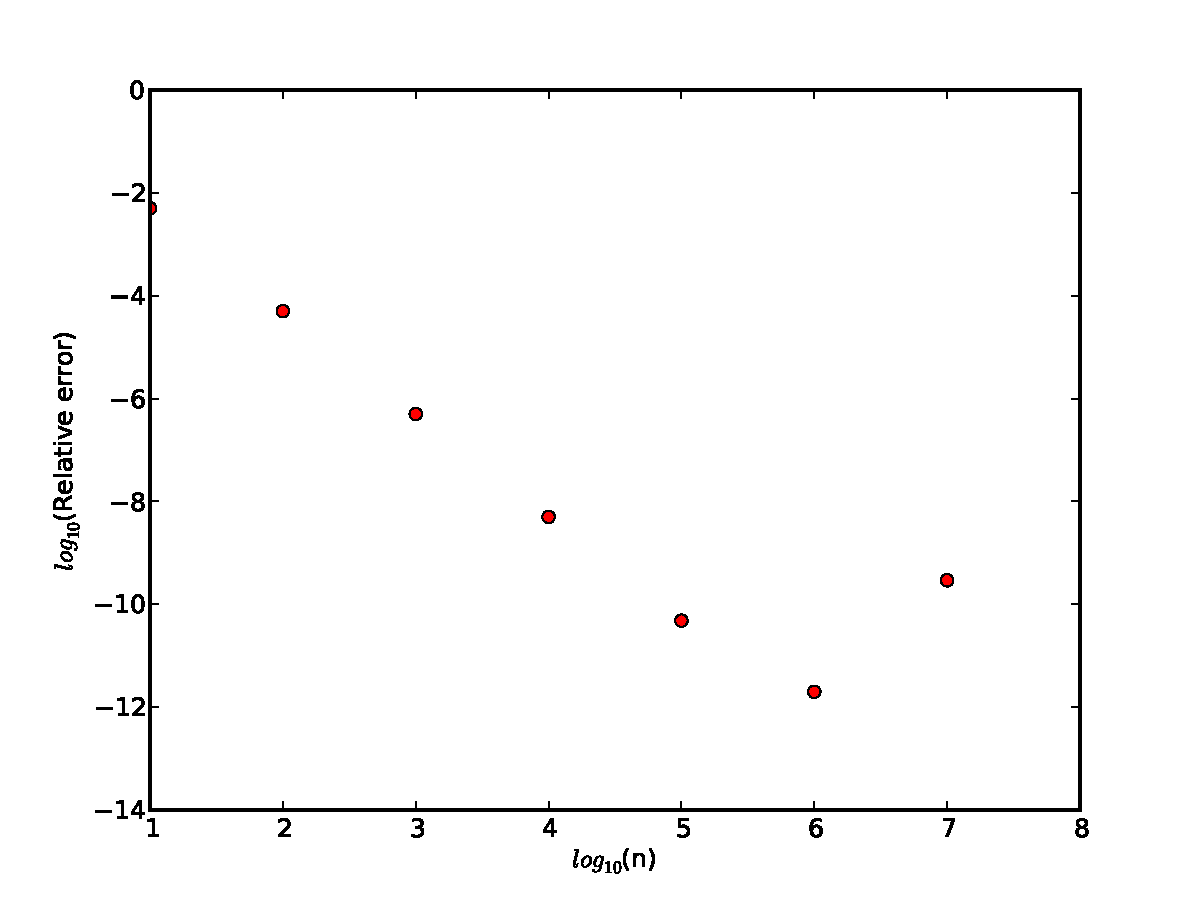
\includegraphics[scale=0.8]{Figures/error.pdf}
\caption{Log-log plot of the relative error as function of the number of integration points. Till approximately $n=10^6$, the relative error follows the predicted mathematical error of the trapezoidal rule. For higher numbers of integration points, numerical round off errors and loss of numerical precision give an increasing relative error.}\label{fig:error}
\end{figure}

The above example allows the student to also test the mathematical
error of the algorithm for the trapezoidal rule by changing the number
of integration points. The students get trained from day one to think
error analysis. Figure \ref{fig:error}  shows clearly the region where the
relative error starts increasing.  The mathematical error which
follows the trapezoidal rule goes as $O(h^2)$ where $h$ is the chosen
numerical step size. It is proportional to the inverse of the number of integration points $n$, that is $h\propto 1/n$.

Before numerical round-off errors and loss of
numerical precision kick in (near $h\sim 10^{-6}$) we see that the
relative error in the log-log plot has a slope which follows the
mathematical error.

There are several additional benefits here. The general learning outcomes on computing can be included as in for example the following ways. We
can easily bake in how to structure a code in terms of
functions and modules, or how to read input data flexibly from the
command line or how to write unit tests etc.  The conventions and
techniques outlined here will save students a lot of time when one
extends incrementally software over time, from simpler to more
complicated problems. In the next subsection we show how algorithms
for solving sets of ordinary differential equations and finding
eigenvalues can be reused in different courses with minor
modifications only.



